\section{TVertex Class Reference}
\label{classTVertex}\index{TVertex@{TVertex}}
Secondary Vertex Class.  


{\tt \#include $<$TVertex.h$>$}

Inheritance diagram for TVertex:\begin{figure}[H]
\begin{center}
\leavevmode
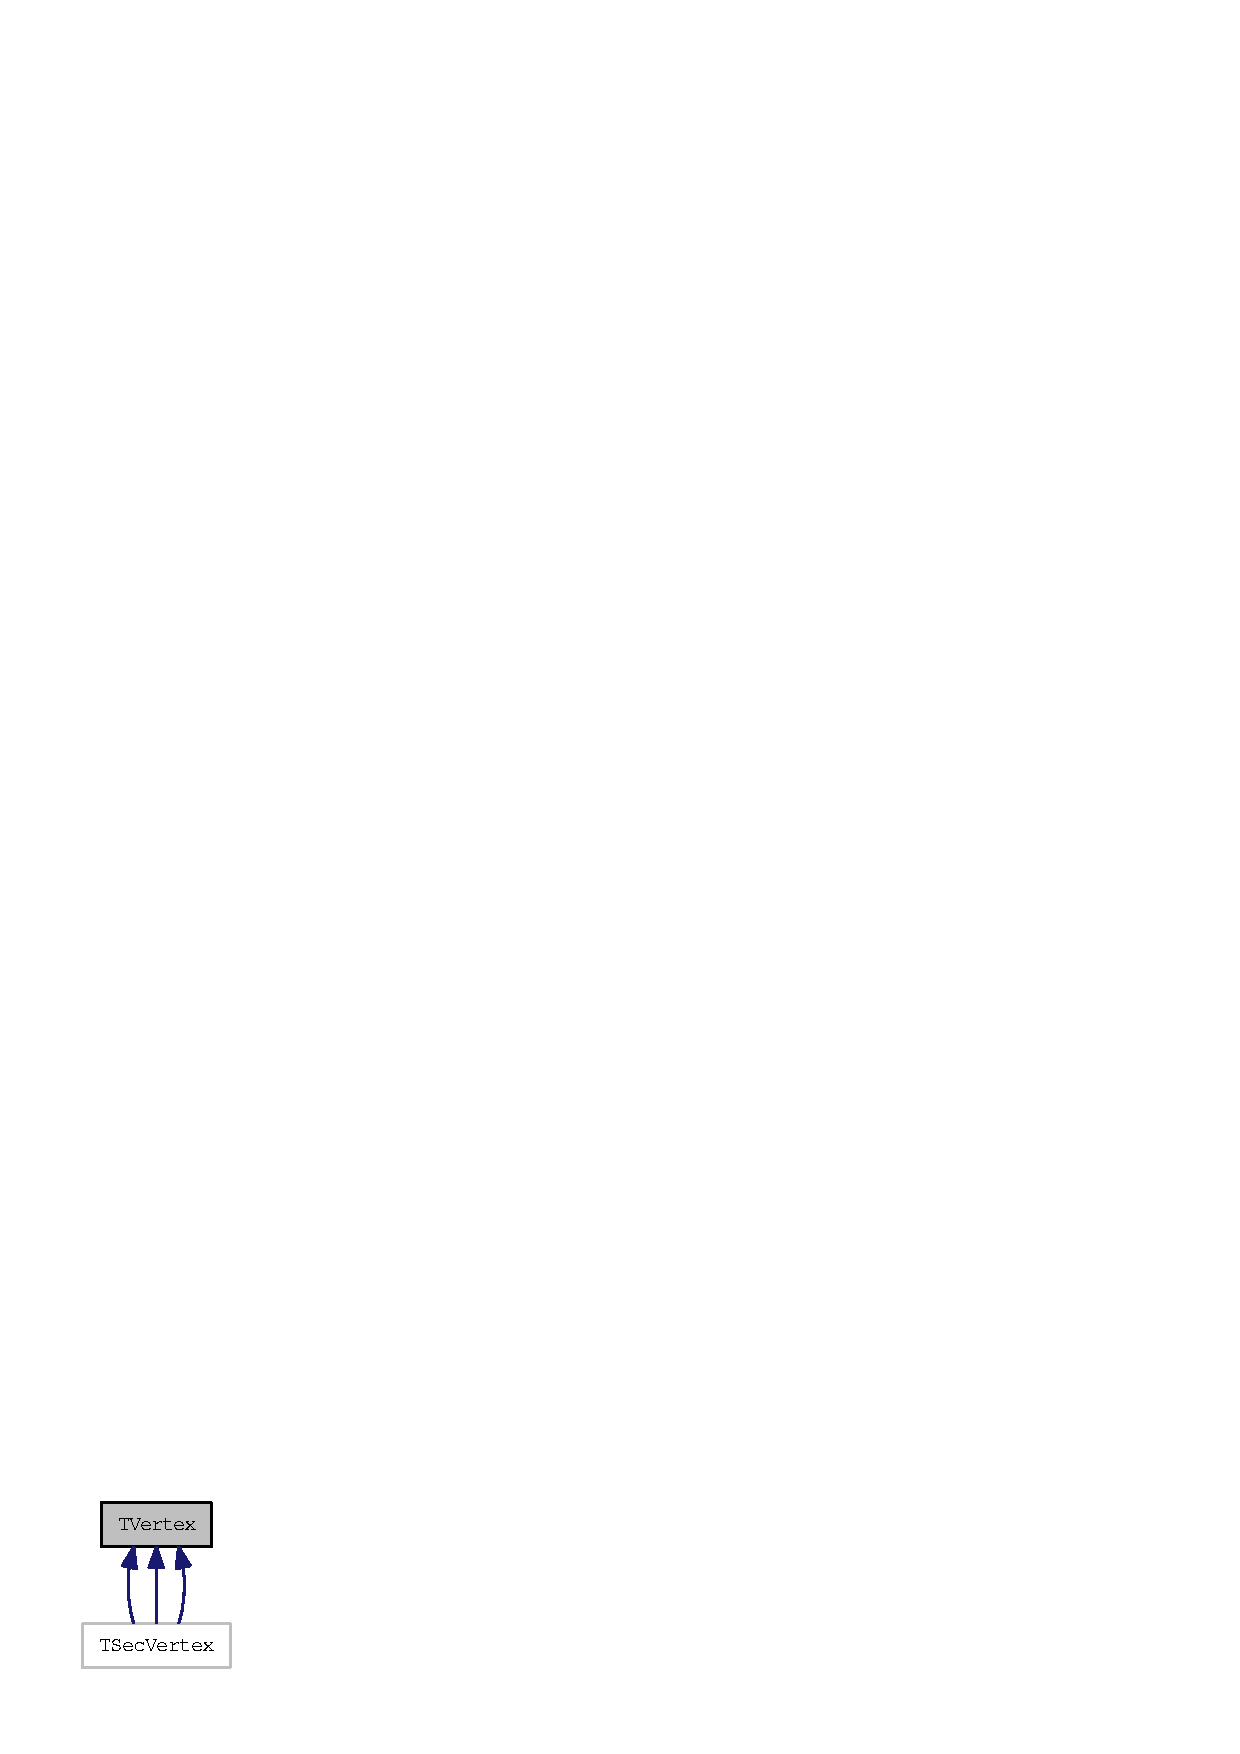
\includegraphics[width=57pt]{classTVertex__inherit__graph}
\end{center}
\end{figure}
\subsection*{Public Member Functions}
\begin{CompactItemize}
\item 
Float\_\-t \bf{Calculate\-Vertex\-Significance} ()
\item 
Float\_\-t \textbf{Calculate\-Vertex\-Projected\-Decay\-Length} ()\label{classTVertex_ecea9b286a92b095932469a7de3aa2bd}

\item 
bool \textbf{Refit\-Vertex} ()\label{classTVertex_c055f1e4fd242af667dc75b2ddc65510}

\item 
void \textbf{Set\-Vertex\-Coordinates} (Float\_\-t x, Float\_\-t y, Float\_\-t z)\label{classTVertex_16b8e7d29d338575a2a41e12d367c9b9}

\item 
void \textbf{Set\-Primary\-Vertex\-Coordinates} (Float\_\-t x, Float\_\-t y, Float\_\-t z)\label{classTVertex_d4d2a41f241a55909bb05c108c7964f2}

\item 
void \textbf{Set\-Primary\-Vertex\-Coordinates\-Error} (Float\_\-t xerr, Float\_\-t yerr, Float\_\-t zerr)\label{classTVertex_97aed75fcd394567e0948054645c62b2}

\item 
void \textbf{Set\-Axis\-Vector} (Float\_\-t eta, Float\_\-t phi)\label{classTVertex_fc11fe48446ef2441e3a234d69dad05e}

\item 
void \textbf{Set\-Vertex\-Covariance} (Float\_\-t $\ast$cov)\label{classTVertex_645430c92c46a8f846a5059e785b52dc}

\item 
void \textbf{Set\-Vertex\-Tracks} (Int\_\-t ntracks, Int\_\-t $\ast$track\-IDs)\label{classTVertex_9954866c3bc36cbc51db8c9a86498aa2}

\item 
void \textbf{Set\-Track\-Parameters} (Int\_\-t ntracks, Float\_\-t helices[30][5], Float\_\-t helixcov[30][15], Float\_\-t $\ast$trackmom)\label{classTVertex_64717d6257025b0530ef666d8fb88bf9}

\item 
void \textbf{Set\-Track\-Pt} (Int\_\-t ntracks, Float\_\-t $\ast$trackp\-T)\label{classTVertex_7130aa75c60198f05e60932f7b257ebd}

\item 
void \textbf{Set\-Apply\-Smearing} (bool applysmearing)\label{classTVertex_cc96dc73f2cf0773835285bf60c201c9}

\item 
void \textbf{Set\-Drop\-Tracks} (bool drop\_\-tracks)\label{classTVertex_ae0c54891a9d25d83b2d64674572c15d}

\item 
void \textbf{Set\-Drop\-Track\-Probability} (Float\_\-t prob)\label{classTVertex_91a2748883e3225c7f09a67fa24b1951}

\item 
void \textbf{Set\-Vertex\-Mass} (Float\_\-t mass)\label{classTVertex_c1fc26d682e76533be9526d502b592c2}

\item 
void \textbf{Set\-Chi2} (Float\_\-t chi2)\label{classTVertex_90221a90bcc1420b4e4a39a9a731c013}

\item 
void \textbf{Set\-NTracks} (Int\_\-t ntracks)\label{classTVertex_70008f032aed4ee1f1a691345b3c6d6f}

\item 
void \textbf{Set\-ZUFO\_\-jet\_\-ratio} (Float\_\-t ZUFO\_\-jet)\label{classTVertex_feb80de531b29a015fe9686e7d1803ad}

\item 
void \textbf{Set\-CAL\_\-total\_\-ratio} (Float\_\-t CAL\_\-total)\label{classTVertex_78e5972ecc19f970282fef3377e1b763}

\item 
void \textbf{Set\-ZUFO\_\-type} (Int\_\-t type)\label{classTVertex_67601944eb1a21b61efb277c862a4d80}

\item 
void \textbf{Get\-Track\-Parameters} (Int\_\-t \&ntracks, Float\_\-t helices[30][5], Float\_\-t helixcov[30][15], Float\_\-t $\ast$trackmom)\label{classTVertex_c61fb892d9fcceb6de702e42d25609c9}

\item 
void \textbf{Get\-Track\-Pt} (Float\_\-t $\ast$trackp\-T)\label{classTVertex_f44f9b081d55afa045fb91762d591cfc}

\item 
void \textbf{Get\-Vertex\-Coordinates} (Float\_\-t \&x, Float\_\-t \&y, Float\_\-t \&z)\label{classTVertex_5f33234c0d8284ebf4028ca38015b5c6}

\item 
Float\_\-t $\ast$ \textbf{Get\-Vertex\-Covariance} ()\label{classTVertex_3a9f670bad415783d500e28c65d5dd05}

\item 
void \textbf{Get\-Vertex\-Tracks} (Int\_\-t \&ntracks, Int\_\-t $\ast$track\-IDs)\label{classTVertex_089a50110ef5368275481901718d529e}

\item 
Float\_\-t \textbf{Get\-Vertex\-Mass} ()\label{classTVertex_c94ae1f4516ce154c1b3ed768e457719}

\item 
Float\_\-t \textbf{Get\-Vertex\-Significance} ()\label{classTVertex_296ef06acc017382c7f8dc3b7a1f8bcc}

\item 
Float\_\-t \textbf{Get\-Vertex\-Projected\-Decay\-Length} ()\label{classTVertex_55efa6467bd6c17c20f5d12506355a1f}

\item 
Float\_\-t \textbf{Get\-Vertex\-Projected\-Decay\-Length\-Error} ()\label{classTVertex_80751606fe403a6b33de6c911ba67501}

\item 
Float\_\-t \textbf{Get\-Vertex\-Decay\-Length} ()\label{classTVertex_32088f262eaa102e1b88d6308c71941c}

\item 
Float\_\-t \textbf{Get\-Axis\-Phi} ()\label{classTVertex_13d0b88a1cf1403852b77a0dc174a6f9}

\item 
Float\_\-t \textbf{Get\-Axis\-Eta} ()\label{classTVertex_e42e7665bee94c8179530de34a23df58}

\item 
Float\_\-t \textbf{Get\-Primary\-Vertex\-XError} ()\label{classTVertex_846e51f6d8f247cdb4983949aa2b4c06}

\item 
Float\_\-t \textbf{Get\-Primary\-Vertex\-YError} ()\label{classTVertex_b5b578eff7dff8b302dded7842f6e358}

\item 
Float\_\-t \textbf{Get\-Primary\-Vertex\-Coordinate\-X} ()\label{classTVertex_d233c4c2c05c752c0acd6f8a340dde94}

\item 
Float\_\-t \textbf{Get\-Primary\-Vertex\-Coordinate\-Y} ()\label{classTVertex_50a08588735755d676121b4f6b88ed3c}

\item 
Float\_\-t \textbf{Get\-Primary\-Vertex\-Coordinate\-Z} ()\label{classTVertex_88e81de9682f142b79530055f2b77b74}

\item 
Int\_\-t \textbf{Get\-NTracks} ()\label{classTVertex_22264dcc175c0ab02ea4222201a851c1}

\item 
unsigned \textbf{Get\-NTracks\-Dropped} ()\label{classTVertex_e44861681b2f995541d0eb147ea78209}

\item 
Float\_\-t \textbf{Get\-Chi2} ()\label{classTVertex_eebd0ba6a2f24d745dee77727a514e1b}

\item 
Float\_\-t \textbf{Get\-ZUFO\_\-jet\_\-ratio} ()\label{classTVertex_9dd0cc3f2f189d5f1ce29dddd4ea7bef}

\item 
Float\_\-t \textbf{Get\-CAL\_\-total\_\-ratio} ()\label{classTVertex_27db208e6bd1e11b4b602b8f1f9a2e9c}

\item 
Int\_\-t \textbf{Get\-ZUFO\_\-type} ()\label{classTVertex_e1222d133d8b4b26a8cfc43cb68515f0}

\item 
void \textbf{Print} ()\label{classTVertex_139e7de94a425d2c97a0d8d8006d1cba}

\item 
\textbf{TVertex} (double ax, double ay, double az)\label{classTVertex_68c048d3c4adf5db80da0a63167d920c}

\item 
void \textbf{Set\-NTracks} (int antracks)\label{classTVertex_6055513ece070c2367ef84e9d6eff498}

\item 
void \textbf{Set\-Chi2} (const double \&achi2)\label{classTVertex_030cf7d93fe6d871b0ac78fe751b29bd}

\item 
void \textbf{Set\-Ndf} (const double \&andf)\label{classTVertex_a190c8dd6ca8e8789149d1556541c7b9}

\item 
int \textbf{NTracks} ()\label{classTVertex_06e89217c8f6756bdd2aaa3f0a870ed4}

\item 
double \textbf{Chi2} ()\label{classTVertex_dbedf19276ec1d01662c98c32742dfc2}

\item 
double \textbf{Ndf} ()\label{classTVertex_51885e0e598abdc758f44c85b2653ba2}

\item 
\textbf{TVertex} (double ax, double ay, double az)\label{classTVertex_68c048d3c4adf5db80da0a63167d920c}

\item 
void \textbf{Set\-NTracks} (int antracks)\label{classTVertex_6055513ece070c2367ef84e9d6eff498}

\item 
void \textbf{Set\-Chi2} (const double \&achi2)\label{classTVertex_030cf7d93fe6d871b0ac78fe751b29bd}

\item 
void \textbf{Set\-Ndf} (const double \&andf)\label{classTVertex_a190c8dd6ca8e8789149d1556541c7b9}

\item 
int \textbf{NTracks} ()\label{classTVertex_06e89217c8f6756bdd2aaa3f0a870ed4}

\item 
double \textbf{Chi2} ()\label{classTVertex_dbedf19276ec1d01662c98c32742dfc2}

\item 
double \textbf{Ndf} ()\label{classTVertex_51885e0e598abdc758f44c85b2653ba2}

\item 
\textbf{TVertex} (double ax, double ay, double az)\label{classTVertex_68c048d3c4adf5db80da0a63167d920c}

\item 
void \textbf{Set\-NTracks} (int antracks)\label{classTVertex_6055513ece070c2367ef84e9d6eff498}

\item 
void \textbf{Set\-Chi2} (const double \&achi2)\label{classTVertex_030cf7d93fe6d871b0ac78fe751b29bd}

\item 
void \textbf{Set\-Ndf} (const double \&andf)\label{classTVertex_a190c8dd6ca8e8789149d1556541c7b9}

\item 
int \textbf{NTracks} ()\label{classTVertex_06e89217c8f6756bdd2aaa3f0a870ed4}

\item 
double \textbf{Chi2} ()\label{classTVertex_dbedf19276ec1d01662c98c32742dfc2}

\item 
double \textbf{Ndf} ()\label{classTVertex_51885e0e598abdc758f44c85b2653ba2}

\end{CompactItemize}
\subsection*{Public Attributes}
\begin{CompactItemize}
\item 
Int\_\-t \textbf{id}\label{classTVertex_805f605f178abc261140709e3e6f770f}

\item 
Int\_\-t \textbf{f\-Jet\-B}\label{classTVertex_4fb81914f7d6bcdab3f67639ee775155}

\item 
Float\_\-t \textbf{Proj\-Decay\-Length}\label{classTVertex_b2549b160cb26f10fc82f25255eb657c}

\item 
Float\_\-t \textbf{Proj\-Decay\-Length\-Error}\label{classTVertex_2728aa1a4ff5a57a76625b3f5dce89a4}

\item 
Float\_\-t \textbf{Significance}\label{classTVertex_0db0fea7037cd98ae235547a0207ffd9}

\item 
Float\_\-t \textbf{chi2ndf}\label{classTVertex_271dac30c657c4610c65a0b309461239}

\item 
Int\_\-t \textbf{f\-Track\-List} [30]\label{classTVertex_1e59075d9a7e15afec83aad023ad63ce}

\end{CompactItemize}
\subsection*{Static Public Attributes}
\begin{CompactItemize}
\item 
static TRandom3 \textbf{rnd}\label{classTVertex_ba84d3452d6ae677fa3959873eb03026}

\item 
static TRandom3 \textbf{rnd2}\label{classTVertex_bebc378ecb14016346b3fed32854f50b}

\item 
static TRandom3 \textbf{f\-Rnd\-Drop\-Tracks}\label{classTVertex_618b3a02f8f5fdd447577f84e03cd0e9}

\item 
static unsigned \textbf{two\_\-track\_\-vertices\_\-total} = 0\label{classTVertex_32f6b18733f286a647b43b967c13c066}

\item 
static unsigned \textbf{two\_\-track\_\-vertices\_\-dropped} = 0\label{classTVertex_74f1a12bed36ce992a0c8c68404620a7}

\end{CompactItemize}
\subsection*{Private Attributes}
\begin{CompactItemize}
\item 
Float\_\-t \bf{f\-Significance}\label{classTVertex_4ee0371ab0fed7f2e5db0f4c3d1943a8}

\begin{CompactList}\small\item\em significance of the vertex \item\end{CompactList}\item 
Float\_\-t \bf{f\-Proj\-Decay\-Length}\label{classTVertex_ec3cfaf6d692894a5c32c8c6f3910a30}

\begin{CompactList}\small\item\em projected decay length of the vertex \item\end{CompactList}\item 
Float\_\-t \bf{f\-Significance\-Smeared}\label{classTVertex_05bc5b68cf637633460db952db2add97}

\begin{CompactList}\small\item\em significance of the vertex after the smearing \item\end{CompactList}\item 
Float\_\-t \bf{f\-Proj\-Decay\-Length\-Smeared}\label{classTVertex_107d54a1efeaec72b60c968cda307b68}

\begin{CompactList}\small\item\em projected decay length of the vertex after smearing \item\end{CompactList}\item 
Float\_\-t \bf{f\-Vertex\-X}\label{classTVertex_1b9d4292cc6634c40bd75771403273fa}

\begin{CompactList}\small\item\em X coordinate of the vertex. \item\end{CompactList}\item 
Float\_\-t \bf{f\-Vertex\-Y}\label{classTVertex_a9983a42727ce998dc121f2842e5a3f5}

\begin{CompactList}\small\item\em Y coordinate of the vertex. \item\end{CompactList}\item 
Float\_\-t \bf{f\-Vertex\-Z}\label{classTVertex_3f5c1448760204b5887a64a3d59f2a82}

\begin{CompactList}\small\item\em Z coordinate of the vertex. \item\end{CompactList}\item 
Float\_\-t \bf{f\-Vertex\-Covariance} [6]\label{classTVertex_c6a478e22ba5b538b2df318a6a713245}

\begin{CompactList}\small\item\em Array containing to covariance matrix of the vertex. \item\end{CompactList}\item 
Float\_\-t \bf{f\-Primary\-Vertex\-X}\label{classTVertex_22131d10d49d69d72d80c62f5d47bc21}

\begin{CompactList}\small\item\em X coordinate of the primary vertex (= beam spot X). \item\end{CompactList}\item 
Float\_\-t \bf{f\-Primary\-Vertex\-Y}\label{classTVertex_43ae65e3e888dbc1bcf000875ca6dd72}

\begin{CompactList}\small\item\em Y coordinate of the primary vertex (= beam spot Y). \item\end{CompactList}\item 
Float\_\-t \bf{f\-Primary\-Vertex\-Z}\label{classTVertex_9542a039c83ef6001b229e6f510fad5f}

\begin{CompactList}\small\item\em Z coordinate of the primary vertex (= reduced primary Z). \item\end{CompactList}\item 
Float\_\-t \bf{f\-Primary\-Vertex\-XError}\label{classTVertex_b7bc0a355feacfb0b02c119dbc951d76}

\begin{CompactList}\small\item\em error on X coordinate of the primary vertex (= beam spot size X) \item\end{CompactList}\item 
Float\_\-t \bf{f\-Primary\-Vertex\-YError}\label{classTVertex_397f063bfe74e1be06e5ff0ae411a55f}

\begin{CompactList}\small\item\em error on Y coordinate of the primary vertex (= beam spot size Y) \item\end{CompactList}\item 
Float\_\-t \bf{f\-Primary\-Vertex\-ZError}\label{classTVertex_d1ac0d03139f5f17dd472b87c76a8608}

\begin{CompactList}\small\item\em error on Z coordinate of the primary vertex (= error on reduced primary Z) \item\end{CompactList}\item 
Float\_\-t \bf{f\-Axis\-Eta}\label{classTVertex_8651dd5f72d0e1a93a16d3d2db6336f1}

\begin{CompactList}\small\item\em eta (pseudorapidity) of the reference axis \item\end{CompactList}\item 
Float\_\-t \bf{f\-Axis\-Phi}\label{classTVertex_fb2dffb6cf9b72b5bab8728dd7451c9c}

\begin{CompactList}\small\item\em phi angle of the reference axis \item\end{CompactList}\item 
Float\_\-t \bf{f\-Mass}\label{classTVertex_a303587bdbe889c4f19d6f75a863ced0}

\begin{CompactList}\small\item\em vertex mass \item\end{CompactList}\item 
Float\_\-t \textbf{f\-Chi2}\label{classTVertex_bba1f42089451fb79461540c52b9cc6d}

\item 
Int\_\-t \textbf{f\-Number\-Of\-Tracks}\label{classTVertex_456fc7dbafa4703c2e38d4d6335ec3a2}

\item 
Int\_\-t \textbf{f\-Track\-IDs} [30]\label{classTVertex_b8f411158223ebf9d697033dfa0d1f85}

\item 
Float\_\-t \textbf{f\-Track\-Helices} [30][5]\label{classTVertex_9d3aec3f9b9b8492cca149de68b93174}

\item 
Float\_\-t \textbf{f\-Track\-Helix\-Covariance} [30][15]\label{classTVertex_ba8a6b7eee13edf9424a1fdbbbd9ad60}

\item 
Float\_\-t \textbf{f\-Track\-Momentum} [30]\label{classTVertex_3edb2ba5ffd100ed6401a794e3824b69}

\item 
Float\_\-t \textbf{f\-Track\-PT} [30]\label{classTVertex_d4c8a732d9aed7c1a35f7b0c6fe16e98}

\item 
bool \textbf{f\-Apply\-Smearing}\label{classTVertex_c7021df951e5f22178c8fc11e91f7fa8}

\item 
bool \textbf{f\-Drop\-Tracks}\label{classTVertex_0a9814c7fef5e2e83e0cf3eb0bad97f9}

\item 
Float\_\-t \textbf{f\-Drop\-Probability}\label{classTVertex_bb658a5b67d7f685ab5228c6a3d42c46}

\item 
unsigned \bf{f\-Tracks\_\-dropped}\label{classTVertex_ac7c645fb686be351e50df99f6690a71}

\begin{CompactList}\small\item\em number of tracks dropped from the fit \item\end{CompactList}\item 
Float\_\-t \textbf{f\-Projected\-Decay\-Length\-Error}\label{classTVertex_37766a7bef01d71f8866e8a85184a5ef}

\item 
Float\_\-t \textbf{f\-Decay\-Length}\label{classTVertex_d0b37678f898bf971717880610184cf7}

\item 
Float\_\-t \textbf{f\-ZUFO\_\-jet\_\-ratio}\label{classTVertex_09ebee49acfe107933f7797b2e1f9e06}

\item 
Float\_\-t \textbf{f\-CAL\_\-total\_\-ratio}\label{classTVertex_d94ac7c290997b57474ae9dfd338ce6c}

\item 
Int\_\-t \textbf{f\-ZUFO\_\-type}\label{classTVertex_0e801712a5ba41151f2b3367297c818c}

\item 
int \textbf{fntracks}\label{classTVertex_d4a1065dbaebb6366b58b4048ca9f073}

\item 
double \textbf{fchi2}\label{classTVertex_9020c3875638aa3afc4c4275399d6c00}

\item 
double \textbf{fndf}\label{classTVertex_5a737cc975692b08e6cc6d88fc09b536}

\end{CompactItemize}


\subsection{Detailed Description}
Secondary Vertex Class. 

This class contains information about single secondary vertex. On one hand it can be used just for storage (as it was before 11/02/2011) On the other hand some operations can be performed (after 11/02/2011): \begin{itemize}
\end{itemize}
Significance calculation from vertex position, reference axis, and beam spot (was done in TMini\-Ntuple\-Analyzer.cxx before) \begin{itemize}
\item Vertex refitting using information track information  \end{itemize}




\subsection{Member Function Documentation}
\index{TVertex@{TVertex}!CalculateVertexSignificance@{CalculateVertexSignificance}}
\index{CalculateVertexSignificance@{CalculateVertexSignificance}!TVertex@{TVertex}}
\subsubsection{\setlength{\rightskip}{0pt plus 5cm}Float\_\-t TVertex::Calculate\-Vertex\-Significance ()}\label{classTVertex_828ec2bd461c898cf280a2a269a8c8ef}




The documentation for this class was generated from the following files:\begin{CompactItemize}
\item 
Ntuple\-Analyzer/inc/TVertex.h\item 
other/final code/TVertex.h\item 
other/final\_\-code/TVertex.h\item 
other/final\_\-code.back/TVertex.h\item 
Ntuple\-Analyzer/src/analysis.cxx\item 
Ntuple\-Analyzer/src/TVertex.cxx\end{CompactItemize}
